\documentclass[a4paper,10pt,landscape,twocolumn]{scrartcl}


\newcommand{\ket}[1]{\lvert #1 \rangle}
\newcommand{\bra}[1]{\langle #1 \rvert}
\newcommand{\id}{\mathbb{I}}

%% Settings
\newcommand\problemset{10}
\newcommand\deadline{Friday November 18th, 20:00h}
\newif\ifcomments
\commentsfalse % hide comments
%\commentstrue % show comments

% Packages
\usepackage[english]{exercises}
%\usepackage{wasysym}
\usepackage{graphicx}
\usepackage{hyperref}
\usepackage{mathabx}
\usepackage{mathrsfs} 
\usepackage{tikz}
\hypersetup{colorlinks=true, urlcolor = blue, linkcolor = blue}

\begin{document}

\practiceproblems

{\sffamily\noindent
%This week's exercises deal with sets, counting and uniform probabilities.
You do not have to hand in these exercises, they are for practicing only. %Problems marked with a $\bigstar$ are generally a bit harder.
}

\begin{exercise}[Position verification with a flawed device]
	Imagine that Alice (one of the verifiers in a position-verification protocol) is unable to prepare BB84 states. Instead, she can only produce qubits in the standard basis $\{\ket0, \ket1\}$ and the Breidbart basis $\{\ket{0_B}, \ket{1_B}\}$, where $\ket{0_B} = \cos(\pi/8)\ket0 + \sin(\pi/8)\ket1$, and $\ket{1_B} = \sin(\pi/8)\ket0 -\cos(\pi/8)\ket1$.
	\begin{subex}
		Drawing on your intuition, do you think it will become easier or harder for dishonest Waldo and Wenda to trick Alice and Bob? Or does it not matter?
	\end{subex}
	\begin{subex}
		Now explicitly compute the probability that dishonest Waldo and Wenda can cheat if Alice sends $n = 1$ qubit (encoded in either the standard or the $\pi/8$ basis with probability 1/2).
	\end{subex}
	\begin{subex}
		Suppose Waldo and Wenda have no quantum memory. What is their winning probability of Alice sends $n$ qubits?
	\end{subex}
\end{exercise}

\begin{exercise}[Personalized position verification]
	Let's imagine Alice and Bob want something more than just position verification. Say they not only want to know that someone is at a given location but also that that person is specifically Waldo, and not anyone else (maybe Wenda). We will build a protocol to do just that. In order to identify Waldo, we will assume that Alice, Bob and Waldo share a secret key $k \in \{0,1\}^n$ ahead of time.
	
	Construct a protocol that satisfies the following conditions:
	\begin{description}
		\item[(Correctness)] If Waldo is at the claimed position, then he can convince Alice and Bob of this fact.
		\item[(Security I)] If Waldo is helped by his companion Wenda (with whom he is unentangled), the probability that he can trick Alice and Bob (into thinking that he is at the location while he is not) is exponentially small in $n$.
		\item[(Security II)] Any impostor Willem cannot trick Alice and Bob into believing that he is Waldo at the claimed location except with probability exponentially small in $n$.
	\end{description}
\end{exercise}

\begin{exercise}[Universality of the brickwork state]
	Consider the ``brickwork state", which was claimed in the lectures to be a universal resource for measurement-based quantum computation. In this exercise you will prove its universality. The $n \times m$ brickwork state is defined as a grid of $n$ rows and $m$ columns of $\ket{+}$ states, with CTRL-Z operations applied between the qubits as follows:
	\begin{itemize}
		\item For all $1 \leq i \leq n$ and all $1 \leq j < m$: between qubits $(i,j)$ and $(i,j+1)$ (the horizontal connections)
		\item For all odd $1 \leq i \leq n$: and all $j \equiv 3 \mod 8$: between qubits $(i,j)$ and $(i+1,j)$, and also between qubits $(i, j+2)$ and $(i+1,j+2)$.
		\item For all even $1 \leq i \leq n$: and all $j \equiv 7 \mod 8$: between qubits $(i,j)$ and $(i+1,j)$, and also between qubits $(i, j+2)$ and $(i+1,j+2)$.
	\end{itemize}
	See also the image below, where the edges represent CTRL-Z operations.
	\begin{center}
	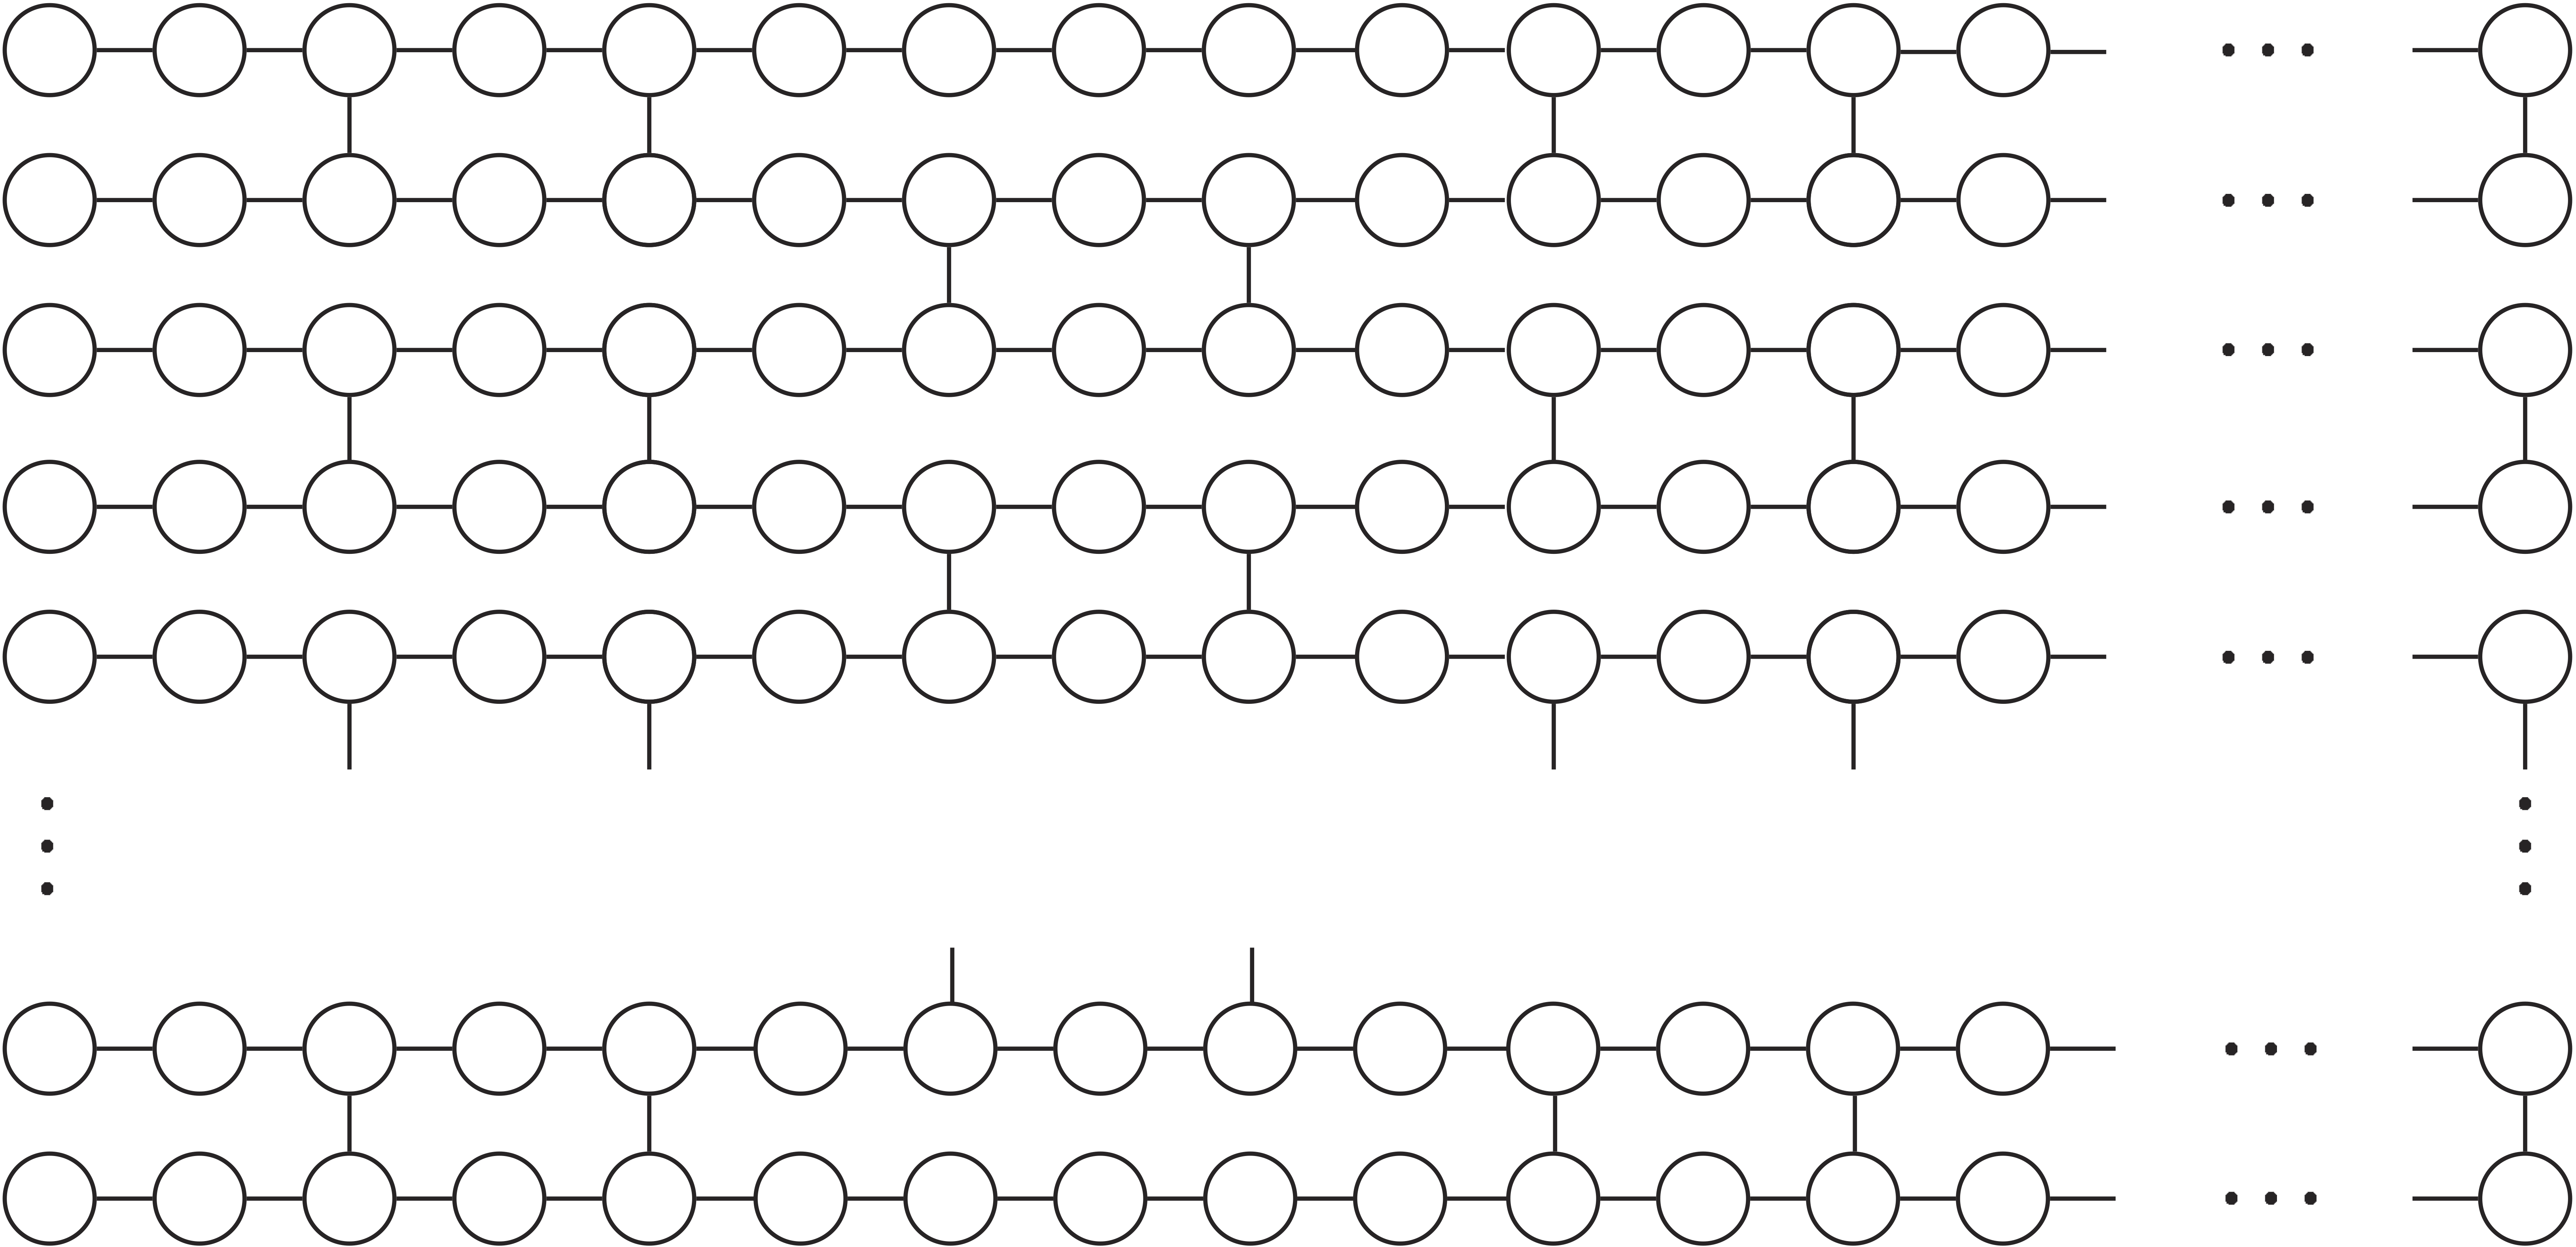
\includegraphics[width=\columnwidth]{10-practice-img1.png}
	\end{center}
	Let $M^{\theta}$ denote the single-qubit measurement in the basis $\{\ket{+_{\theta}}, \ket{-_\theta}\}$, where $\ket{+_{\theta}} = \frac{1}{\sqrt{2}}(\ket0 + e^{i\theta}\ket1)$ and $\ket{-_{\theta}} = \frac{1}{\sqrt{2}}(\ket0 - e^{i\theta}\ket1)$.
	\begin{subex}
		Starting with the state $\ket{\psi} \otimes \ket{+}$, and performing a control-Z followed by a measurement $M^\theta$ on the first qubit, what is the state $\ket{\psi'}$ of the second qubit? Assume the measurement outcome is $\ket{+_{\theta}}$.
		
		Express the unitary that maps $\ket{\psi} \to \ket{\psi'}$ in terms of the Hadamard gate and $U_z(\theta)$, the rotation of $\theta$ around the $z$ axis of the Bloch sphere:
		\[
		U_z(\theta) = \left[\begin{array}{c c}
		1&0\\
		0&e^{i\theta}
		\end{array}\right].
		\]
	\end{subex}
	\begin{subex}
		Show that for any given angle $\theta$ and any Pauli $X^sZ^t$, there exists a $\theta'$ (expressed in terms of $\theta$, $s$, and $t$) such that measuring $M^{\theta'}$ is equivalent to applying $X^sZ^t$ and then measuring $M^{\theta}$. (Here, equivalence is intended in terms of the outcome probabilities and post-measurement state on the remaining qubits. You should assume that the measured qubit is destroyed.)
		
		Conclude that if the measurement outcome was $\ket{-_{\theta}}$ instead of $\ket{+_\theta}$ in the previous subexercise, we can correct the output state to the computed state $\ket{\psi'}$ by measurement only.
	\end{subex}
	\begin{subex}
		Use the result from the previous subexercise to determine the effect of the following \emph{measurement pattern}. The two left-most qubits are the input qubits (in an arbitrary two-qubit pure state $\ket{\psi}$), all other qubits are initialized in the $\ket{+}$ state. The output lands into the only two unmeasured qubits, represented by the two squares.
		
		\begin{center}
			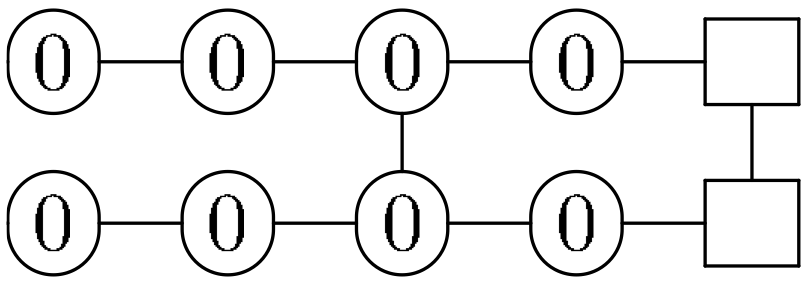
\includegraphics[]{10-practice-img2.png}
		\end{center}
	\end{subex}
	\begin{subex}
		In the above measurement pattern, change \emph{one} measurement angle in order to implement the gate $T \otimes I$.
	\end{subex}
	\begin{subex}
		Which two-qubit unitary is implemented by the following, more general, measurement pattern?
		\begin{center}
			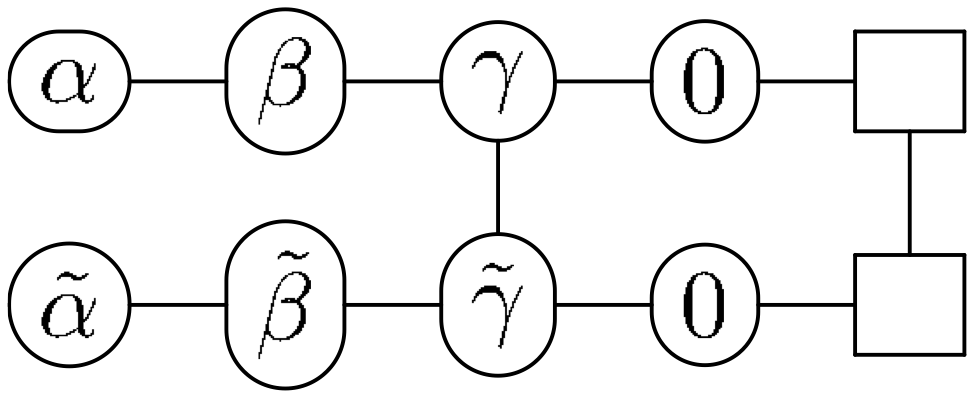
\includegraphics[]{10-practice-img3.png}
		\end{center}
	\end{subex}
	\begin{subex}
		Armed with the knowledge from the previous question, determine which of the following measurement patterns implements a Hadamard gate on the top qubit.
		\begin{center}
			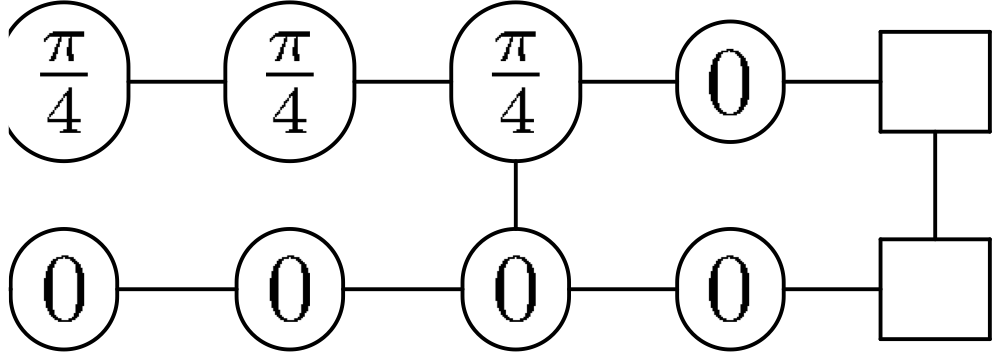
\includegraphics[]{10-practice-img4.png}\qquad
			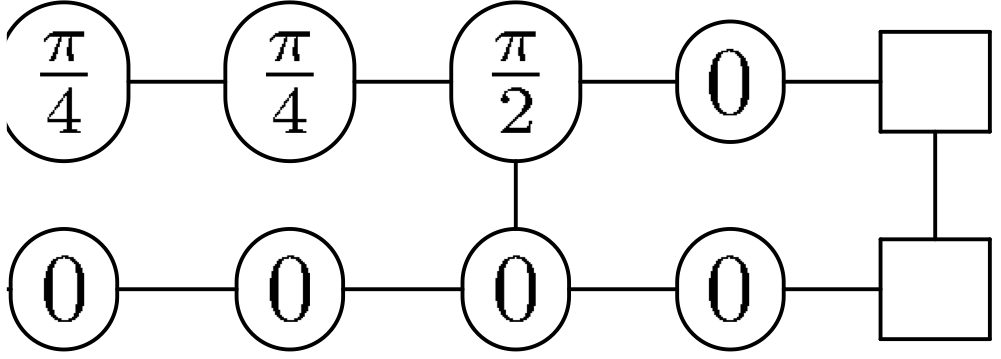
\includegraphics[]{10-practice-img5.png}\\\vspace{1em}
			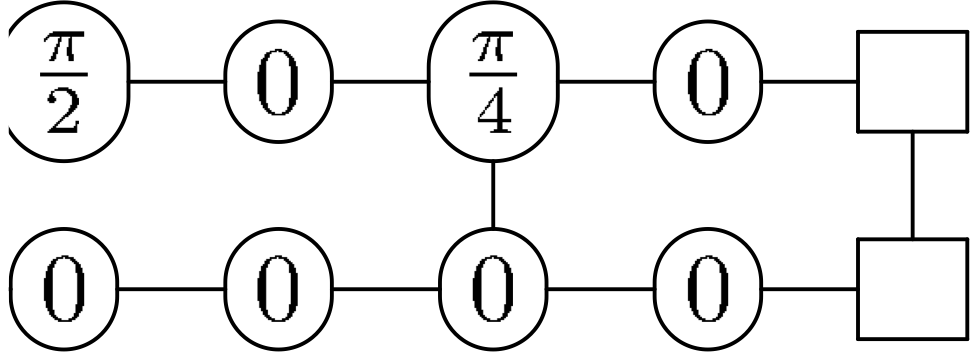
\includegraphics[]{10-practice-img6.png}\qquad
			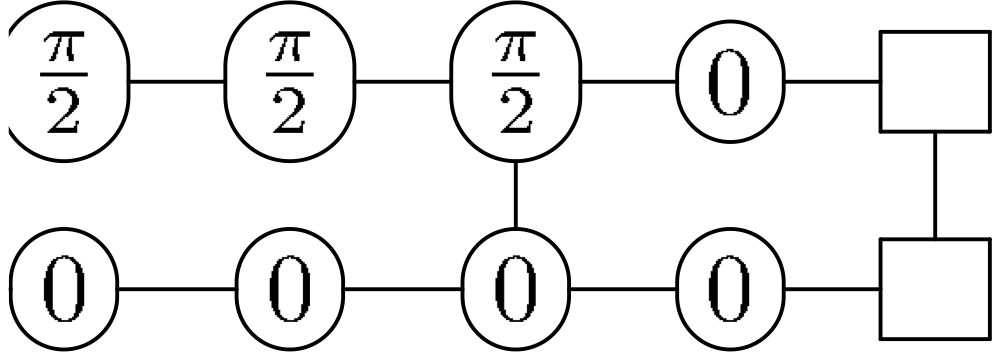
\includegraphics[]{10-practice-img7.png}
		\end{center}
	\end{subex}
	\begin{subex}
		We now know the measurement patterns for $T$ and $H$. For universal quantum computation, we only need to find the pattern for CNOT. Which of the following patterns achieves CNOT with the top qubit as control?
		\begin{center}
			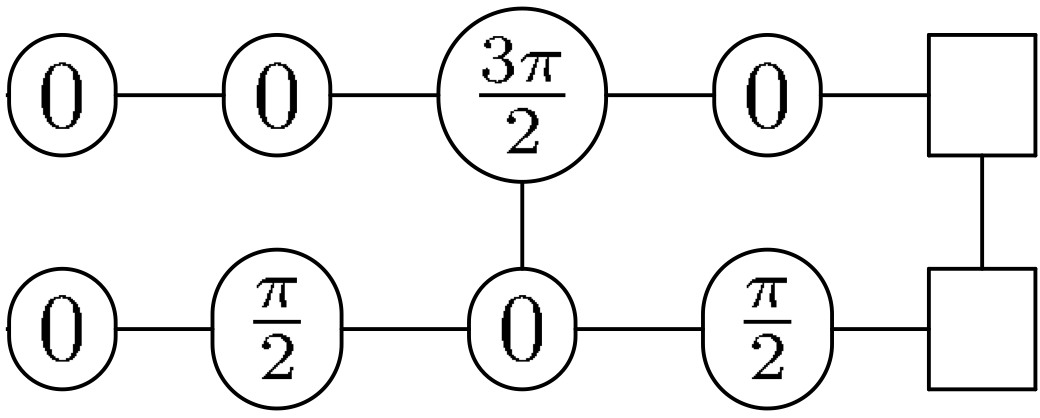
\includegraphics[]{10-practice-img8.png}\qquad
			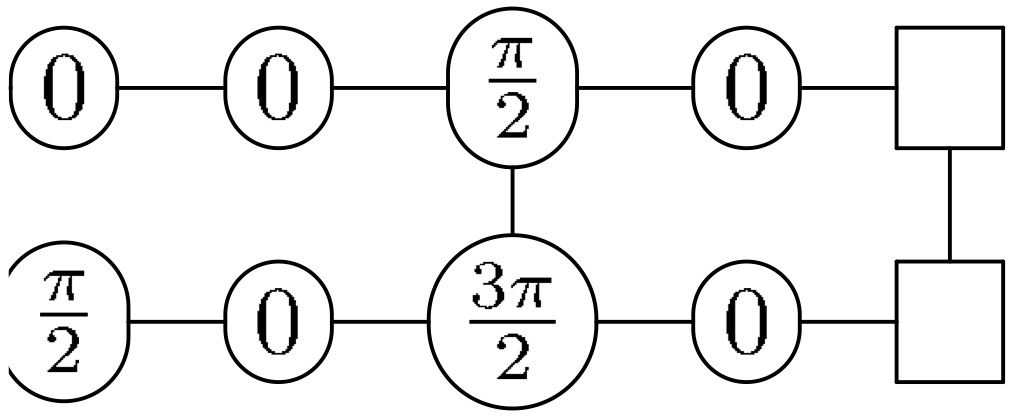
\includegraphics[]{10-practice-img9.png}\\\vspace{1em}
			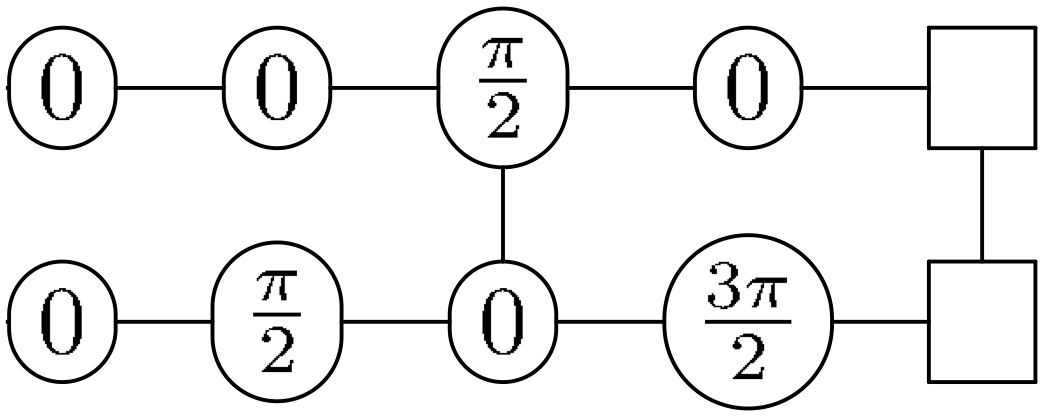
\includegraphics[]{10-practice-img10.png}\qquad
			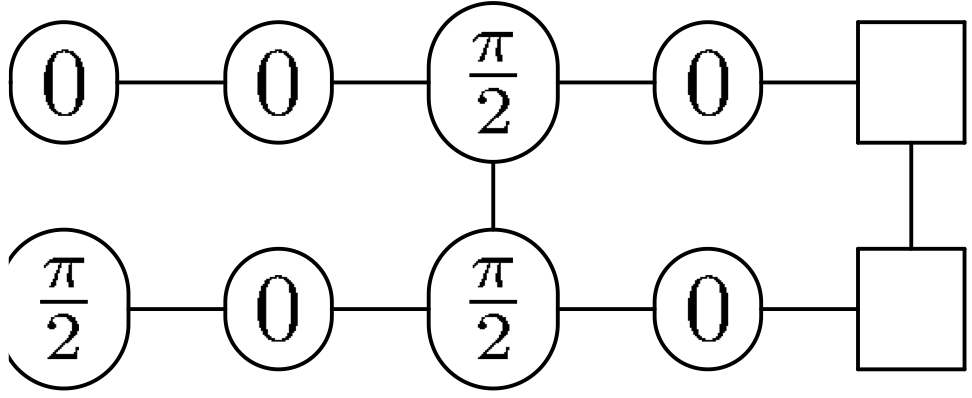
\includegraphics[]{10-practice-img11.png}
		\end{center}
	\end{subex}
	\begin{subex}
		Describe how to perform CNOT between non-adjacent rows in the brickwork state.
	\end{subex}
\end{exercise}


\begin{exercise}[Computing on encrypted quantum data]
	Alice wants Bob to perform some quantum circuit for her. She encrypts her $n$-qubit state using a quantum one-time pad. Call the X-keys $\vec{a} = (a_1, ..., a_n)$ and the Z-keys $\vec{b} = (b_1, ..., b_n)$. She then sends the encrypted state to Bob. In this exercise, you will investigate how Bob can perform the gates $X, Z, H, P, CNOT$, and $T$ on this state in such a way that Alice can, at the end, decrypt the state to the desired outcome: the circuit applied to her input. Bob should not learn anything about Alice's input. During the computation, Alice can perform classical computations on her keys.
	\begin{subex}
		Bob performs the Clifford gates ($X, Z, H, P, CNOT$) by directly applying them to the encrypted qubits. Describe in detail the classical computations Alice must perform to update her keys.
	\end{subex}
	\begin{subex}
		For the rest of this exercise, consider $n = 1$. Let $X^{a}Z^{b}\rho Z^{b}X^{a}$ describe the state of the qubit. Find expressions for $p, x$ and $z$ (in terms of 0, 1, $a$, and $b$) such that
		\[
		TX^{a}Z^{b} = P^pX^xZ^zT.
		\]
	\end{subex}
	\begin{subex}
		$P^p$ is an error on the output state: Bob cannot continue his computation correctly without removing it first. However, Bob does not know $p$ and therefore he cannot perform $(P^p)^{\dagger}$. Should Alice tell him $p$? Why or why not?
	\end{subex}
	%\begin{subex}
	%	Alice and Bob decide to try a different protocol for performing a $T$ gate. Bob does not directly apply the gate to the encrypted state, but instead, he receives an encrypted magic state $X^{a'}Z^{b'}T\ket{+}$ from Alice. He performs the following circuit on the data qubit (top wire) and the magic state (bottom wire):
	%\end{subex}
\end{exercise}












\end{document}